\chapter{Experimental Setup}
\label{ch:exper_setup}
\section{The LHC}
The Large Hadron Collider (\lhc) at \cern is a synchrotron designed to accelerate protons and lead nuclei. This work focuses on the proton-proton collisions during \LHCrunii. During \LHCrunii from 2015 to 2018, the \lhc operated at a centre of mass energy of $\sqrt{s}=13\,\unit{\tera\electronvolt}$ with an integrated luminosity of $\mathcal{L}_{int}\approx 140\,\unit{\femto\barn^{-1}}$ \cite{ATLAS:2019pzw}.

After completion of \LHCruniii in June 2026 and an operational pause, the \lhc will operate with increased luminosity as the High-Luminosity Large Hadron Collider (HL-\lhc). During this phase, it is planned to accumulate data with an integrated luminosity of $\mathcal{L}=3\,\unit{\atto\barn^{-1}}$ \cite{Aberle:2749422}.
 \section{The Detector}
The \atlas detector is a general-purpose particle detector at the \lhc at \cern. It can roughly be separated into three elements: the inner detector, the calorimeter and the muon spectrometer \cite{atlas_tdr}.
\subsection{The Coordinate System}
The interaction point marks the origin of the \atlas coordinate system. The $z$-axis is orientated along the beamline, the $x$-axis points towards the centre of the \lhc and the $y$-axis points upwards.

Using this convention, several kinematic variables are defined. One of which is the transverse momentum defined as
\begin{align}
    p_T=\sqrt{p_x^2+p_y^2}
\end{align}
Because of the cylindrical shape of the \atlas detector and the cylindrical symmetry of the interactions, the azimuthal angle is used as another variable. The polar angle relative to the $z$-axis can be used to define the pseudorapidity which can also be expressed in terms of the momentum
\begin{align}
    \eta=-\ln\left(\tan\left(\frac{\theta}{2}\right)\right)=\ln\left(\frac{|\vec p|+p_z}{|\vec p|-p_z}\right)\,.
\end{align}
In the ultra-relativistic limit $m\ll |\vec p|$ the pseudorapidity is equal to the rapidity defined as
\begin{align}
    y=\frac{1}{2}\ln\left(\frac{E+p_z}{E-p_z}\right)\,.
\end{align}
These variables are convenient for the usage in the \atlas experiment because $p_T,\phi$, and differences of $\eta$ are invariant under Lorentz-boost along the $z$-axis.
\subsection{The Inner Detector}
\begin{figure}[ht]
    \centering
    \includegraphics[width=0.8\textwidth]{figures/atlas-detector/IDbriefing_figure1.png}
    \caption{Schematic cross-section of the inner detector of the \atlas detector (\copyright\ \cern).}
    \label{fig:inner_det}
\end{figure} \noindent
The inner detector (ID) is the innermost part of the \atlas detector. It is used for tracking charged particles, particle identification, and primary and secondary vertex determination \cite{atlas_tdr}. The ID consists of three different sub-detectors. Their rough structure is depicted in \Cref{fig:inner_det}. The ID is encapsulated with a solenoid magnet providing a $2\,\unit{\tesla}$ axial magnetic field on the inside of the ID. The magnetic field is crucial to measure the momentum of a charged particle. The transverse momentum is measured as the curvature of the particle's track due to the Lorentz force.

The detector part closest to the beam pipe is the pixel detector. It consists of 1744 modules arranged in three barrel layers. Each module hosts 47232 silicon pixels with a size of $50\times 400\,\unit{\micro \metre^2}$. The pixels are semiconductor trackers used to detect the traversing of charged particles.

The following part of the detector is the semiconductor tracker (SCT). It consists of 4088 modules arranged in four layers to guarantee four position measurements of charged particles. Each module consists of four silicon sensors. The sensors offer a $17\,\unit{\micro \metre}$ resolution in-plane lateral and $580\,\unit{\micro \metre}$ in-plane longitudinal.

The outermost part of the inner detector is the transition radiation tracker (TRT). It consists of polyimide drift (straw) tubes with a $4\,\unit{\milli\metre}$ diameter that are arranged in a $528\,\unit{\milli\metre}$ thick cylindrical layer around the beam pipe. The straw tubes are interleaved with fibres for the readout. The transition radiation tracker utilizes the transition light emitted by charged particles traversing the interface between two media with different indices of refraction. The TRT offers a measurement of charged particles and electron identification.
\subsection{Calorimeter}
\begin{figure}[ht]
    \centering
    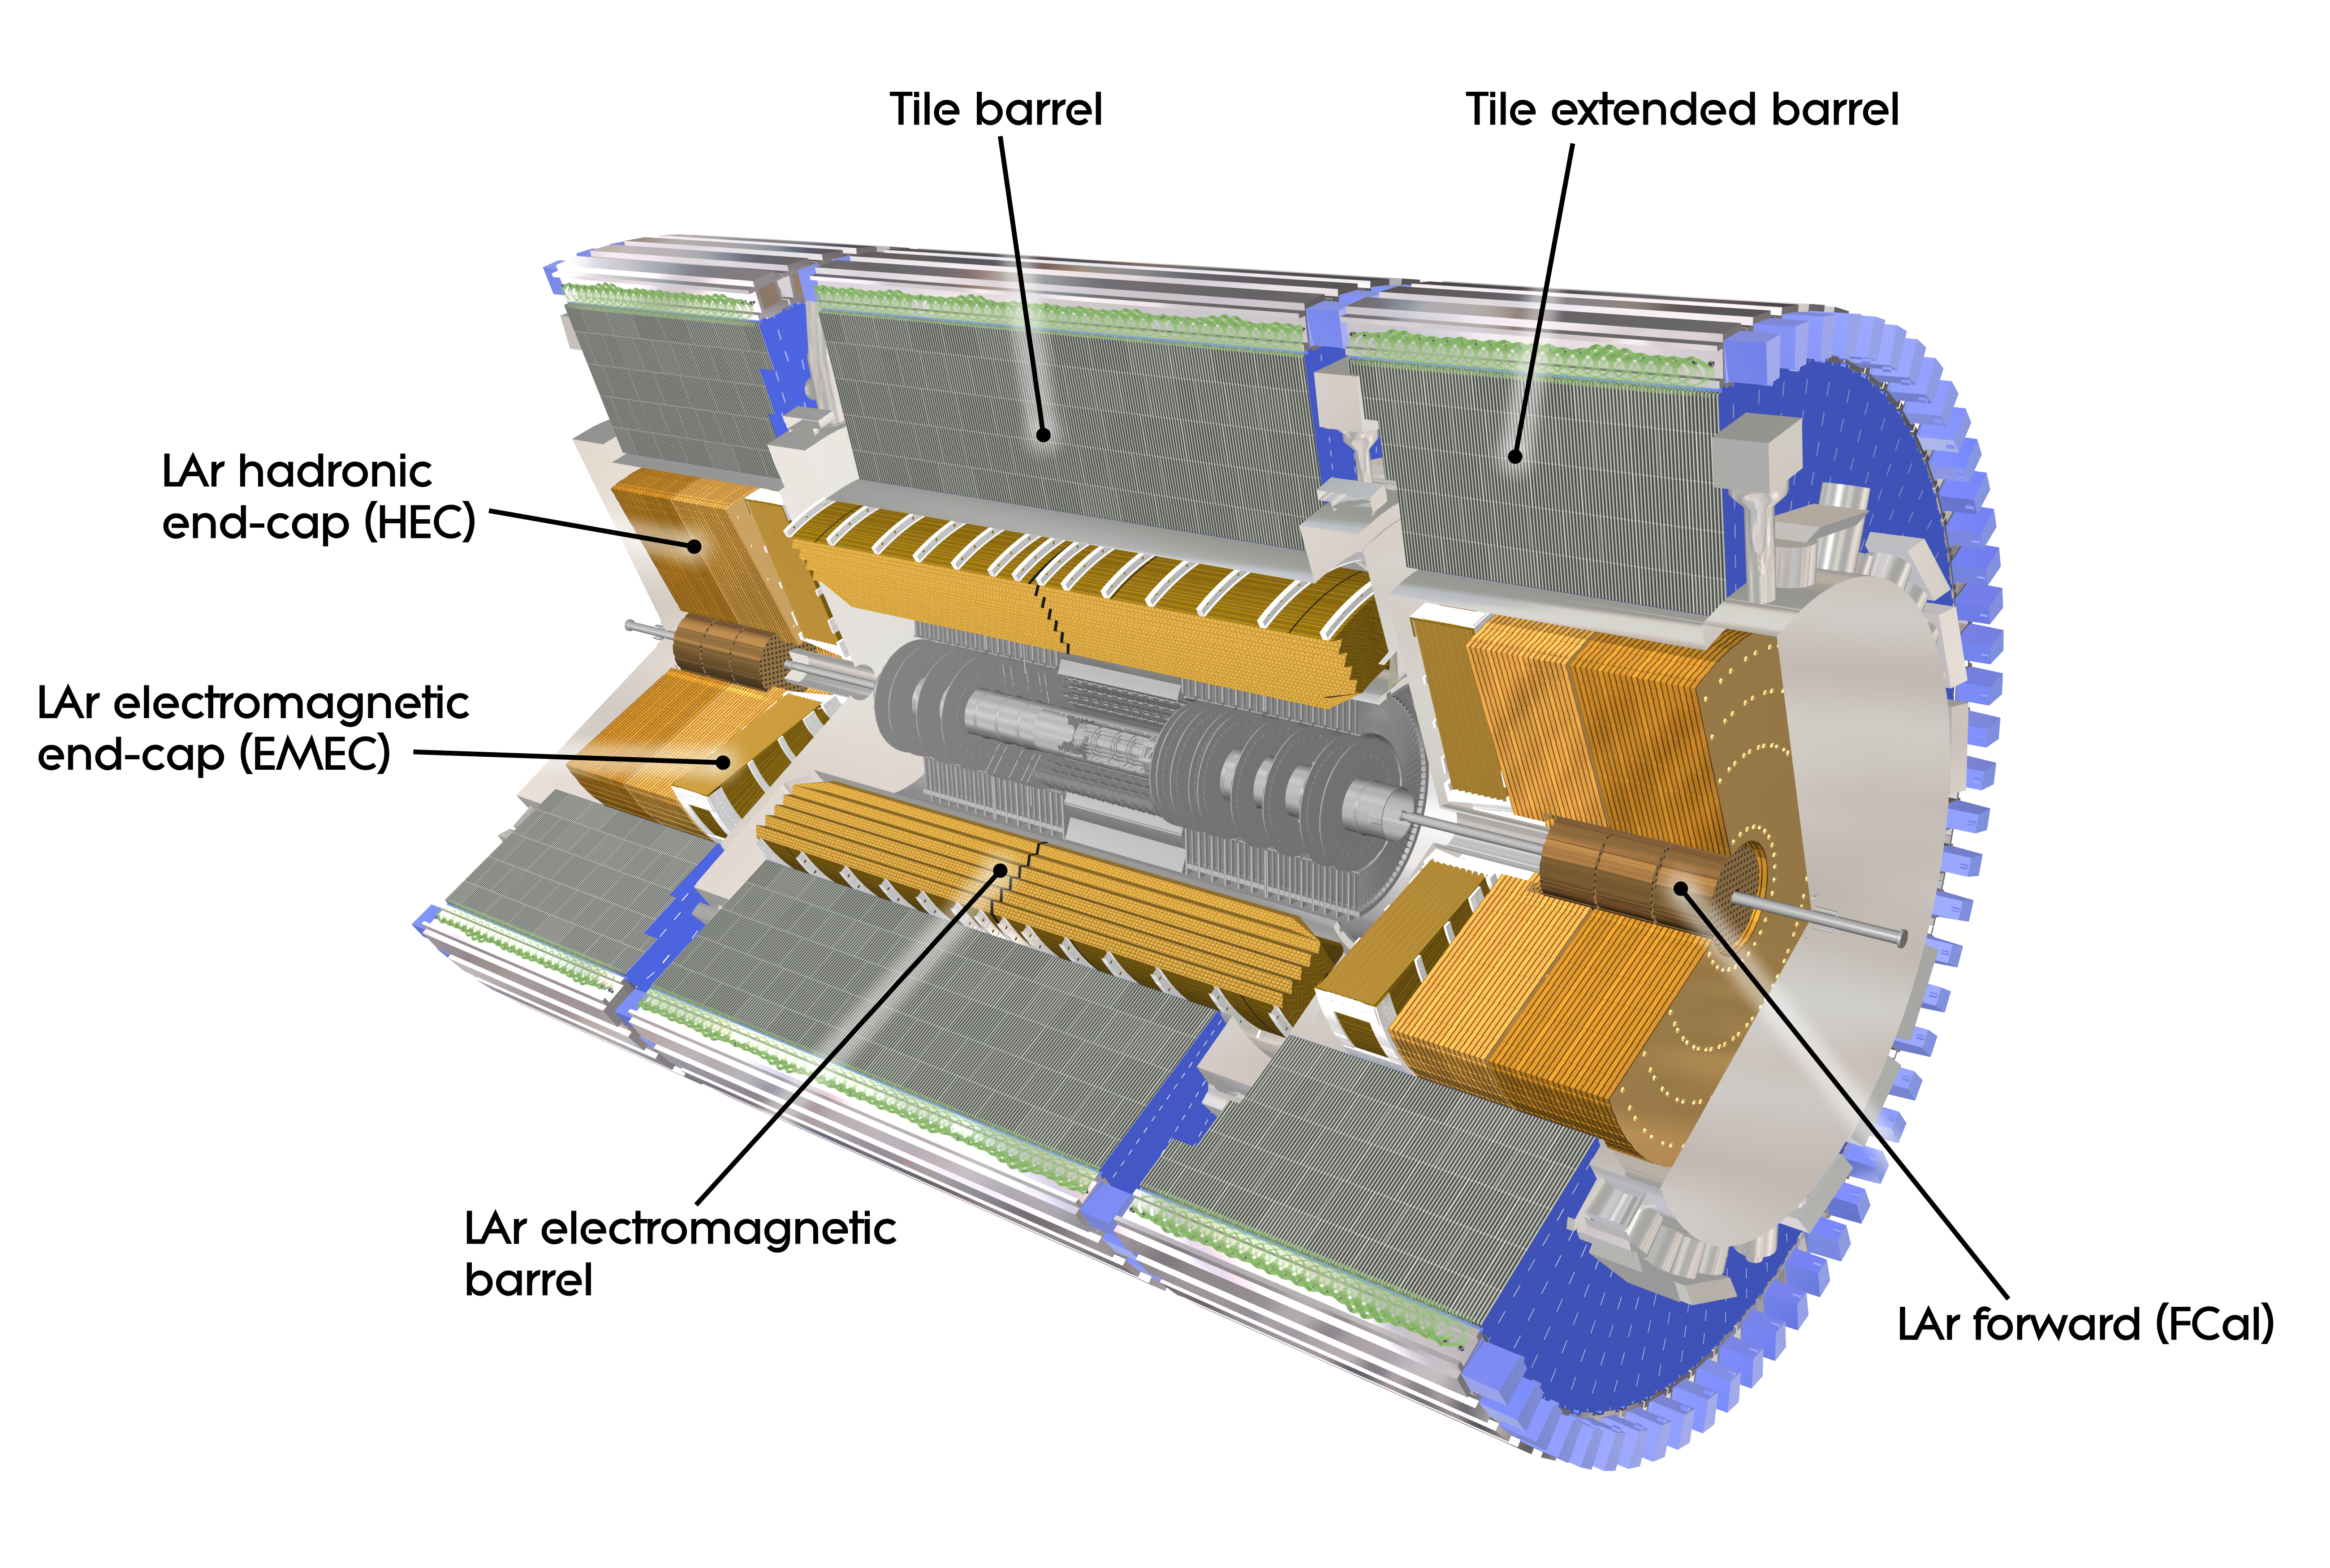
\includegraphics[width=0.7\textwidth]{figures/atlas-detector/0803015_01.jpg}
    \caption{Computer generated image of the \atlas calorimeter (\copyright\ \cern).}
    \label{fig:colorimeter}
\end{figure}\noindent
The calorimeters are the detector layers following the inner detectors. Its structure is divided into the Electromagnetic calorimeter (ECal) and the hadronic calorimeter (HCal).
\subsubsection{Electromagnetic Calorimeter}
The ECal is used for the energy and position measurement of electric charged particles and photons. It utilizes bremsstrahlung and pair production to create a cascade of charged particles which are measured. It offers full azimuthal coverage and is equipped with end caps in the longitudinal direction of the beam pipe. The \atlas ECal is a sampling calorimeter operating with lead as the passive and liquid Argon as the active medium. The innermost part of the ECal is a presampler which detects if the particle started showering before reaching the ECal.
\subsubsection{Hadronic Calorimeter}
The HCal measures the energy and position of baryons and mesons through strong interactions with the nuclei. In the range of $|\eta|<1.7$ it is a sampling calorimeter with steel as the passive and scintillators as the active medium. For the end cap, liquid Argon is deployed as the active medium. The HCal works with the same principle as the ECal but offers less precise measurements.

In the range of $3.1<|\eta|<4.9$ ECal and HCal are substituted with the forward calorimeters (FCal) which are made up of three modules to fulfil the function of both calorimeters.

In combination with the FCal a total range of $|\eta|<4.9$ is covered by the calorimeters.

A computer-generated image of the structure of the different calorimeters used in the \atlas detector is shown in \Cref{fig:colorimeter}.
\subsection{Muon Spectrometer}
The muon spectrometer is the outermost part of the \atlas detector. Its purpose is to detect charged particles exiting the calorimeters and measure their momentum in the range of $|\eta|<2.7$. A detector dedicated to the measurement of muons is necessary because their mass makes them minimal ionizing particles in the energy range of the \lhc collisions. The amount of energy loss due to bremsstrahlung is not sufficient to develop showers necessary to measure their energy. The muons' transverse momenta can be measured in the ID. Like the inner detector, the muon spectrometer utilizes a magnetic field to conduct a measurement of the particle's momentum.  In the muon spectrometer, however, a solenoid magnet is used to allow for the measurement of the muon's momentum along a different direction. Combining the measurements, one obtains full knowledge of the muons four-momentum. Further, does the high rate of stopped electrons and hadrons in the calorimeters enable a high specificity in the muon detection.


\subsection{Trigger System}
With a bunch spacing of $25\,\unit{\nano\second}$ \cite{ATLAS:2019pzw} collisions happen at a rate of $40\,\unit{\mega\hertz}$. Each collision involves up to hundreds of particles. To reduce the data to a feasible amount, triggers are employed to filter less interesting events. Different layers of triggers operate either at the hardware or software level. The L1 trigger is a hardware level trigger and acts as the first filter for the events. It makes decisions in less than $2.5\,\unit{\micro\second}$. The subsequent L2 trigger is a software level trigger and makes decisions in less than $200\,\unit{\micro \second}$. Combined, the trigger system reduces the event rate from $40\,\unit{\mega\hertz}$ to $1000\,\unit{\hertz}$ which are then stored at the \cern data centre.
